\documentclass[10pt,letterpaper]{article}
\usepackage[margin=0.78in,headheight=14pt]{geometry}
\usepackage[T1]{fontenc}
\usepackage[utf8]{inputenc}
\usepackage{lmodern}
\usepackage{microtype}
\usepackage{mathtools,amssymb,amsfonts,bm}
\usepackage{booktabs,longtable,tabularx,array}
\usepackage{siunitx}
\usepackage{graphicx}
\usepackage[table]{xcolor}
\usepackage{tikz}
\usetikzlibrary{arrows.meta,positioning,shapes.geometric,calc}
\usepackage{listings}
\usepackage{enumitem}
\usepackage{fancyhdr}
\usepackage{titlesec}
\usepackage{hyperref}
\usepackage{xurl}
\usepackage{float}
\usepackage{caption}
\usepackage{needspace}
\definecolor{navy}{HTML}{152B49}
\definecolor{teal}{HTML}{007F86}
\definecolor{lightblue}{HTML}{F0F5FA}
\definecolor{pale}{HTML}{E7EDEF}
\definecolor{codebg}{HTML}{F5F7F9}
\hypersetup{colorlinks=true,linkcolor=navy,urlcolor=teal,citecolor=teal,pdftitle={Field-Oriented Control: Theory, Voltage-Mode Modulation, and STM32 Implementation},pdfauthor={James Lavrenz},pdfsubject={Technical note for mtrctrl Phase 2 implementation}}
\setcounter{tocdepth}{1}
\setlength{\parskip}{3.3pt}
\setlength{\parindent}{0pt}
\setlength{\emergencystretch}{2em}
\setlist[itemize]{leftmargin=17pt,itemsep=2pt,topsep=3pt}
\setlist[enumerate]{leftmargin=20pt,itemsep=2pt,topsep=3pt}
\titleformat{\section}{\large\bfseries\color{navy}}{\thesection}{0.65em}{}
\titleformat{\subsection}{\normalsize\bfseries\color{navy}}{\thesubsection}{0.65em}{}
\titleformat{\subsubsection}{\normalsize\bfseries\color{teal}}{\thesubsubsection}{0.65em}{}
\pagestyle{fancy}\fancyhf{}\lhead{\footnotesize\color{navy} mtrctrl / ENGINEERING TECHNICAL NOTE}\rhead{\footnotesize\color{navy} VOLTAGE-MODE FOC}\cfoot{\footnotesize\thepage}
\renewcommand{\headrulewidth}{0.35pt}
\lstdefinestyle{cpp}{backgroundcolor=\color{codebg},basicstyle=\ttfamily\footnotesize,keywordstyle=\color{navy}\bfseries,commentstyle=\color{teal},stringstyle=\color{teal},numbers=left,numberstyle=\tiny\color{gray},numbersep=7pt,breaklines=true,frame=single,framerule=0.3pt,rulecolor=\color{pale},columns=fullflexible,keepspaces=true,tabsize=2,showstringspaces=false}
\lstset{style=cpp}
\newcommand{\Vdc}{V_{\mathrm{dc}}}
\newcommand{\ph}{\mathrm{ph}}
\newcommand{\wrap}{\operatorname{wrap}_{2\pi}}
\newcommand{\sat}{\operatorname{sat}}
\newcommand{\dd}{\mathrm{d}}
\newcommand{\ii}{\mathrm{i}}
\newcommand{\Om}{\omega_m}
\newcommand{\Oe}{\omega_e}
\newcommand{\te}{\theta_e}
\newcommand{\tm}{\theta_m}
\newcommand{\note}[1]{\par\medskip\noindent\colorbox{lightblue}{\parbox{0.965\linewidth}{\textbf{Engineering note.} #1}}\par\medskip}
\begin{document}
\begin{center}
{\Large\bfseries\color{navy} FIELD-ORIENTED CONTROL OF THREE-PHASE\\ PERMANENT-MAGNET MOTORS}\\[8pt]
{\large Theory, Voltage-Mode Modulation, and an STM32F446RE Implementation}\\[10pt]
{\normalsize \textbf{Technical Note TN-FOC-001} \quad Revision 1.0 \quad 26 October 2026}\\[4pt]
{\small James Lavrenz \quad | \quad \texttt{jameslavrenz/mtrctrl} \quad | \quad Design reference for Phase 2}
\end{center}
\vspace{5pt}\hrule\vspace{9pt}
\textbf{Abstract.}\quad This note develops rotor-oriented control of a three-phase permanent-magnet synchronous motor from its electromagnetic and electromechanical equations, with explicit coordinate conventions and an implementation of \emph{voltage-controlled} field-oriented control (FOC): sensor-based electrical angle, $u_d^*=0$, commanded $u_q^*$, inverse Park and Clarke transforms, pulse-width modulation (PWM), and an outer speed controller. The derivation distinguishes commanded voltage from measured current and therefore does not mistake voltage-mode FOC for closed-loop torque control. The implementation discussion is specialized to an STM32 NUCLEO-F446RE, a seven-pole-pair DFRobot FIT1035 with AS5600 encoder, and the DRI0058 three-PWM inverter interface, while remaining generally applicable to microcontrollers. It includes modulation bounds, discrete-time equations, synchronization, startup alignment, pseudocode, verification, and failure analysis. Equations use \emph{peak-valued, amplitude-invariant} Clarke/Park transforms throughout.

\textbf{Scope and status.}\quad This is a mathematical and implementation design note, \textbf{not} evidence of a built or validated Phase 2 drive. The repository's present Phase 1 controls a \emph{simulated} mechanical plant at \SI{100}{Hz}. Any current, voltage, timing, or pin value identified as an \emph{example} is not a tested electrical configuration. The DRI0058 provides no phase-current feedback through the specified interface; current-controlled FOC requires additional hardware.

\makeatletter
\renewcommand*\l@section{\@dottedtocline{1}{0em}{2.0em}}
\makeatother
{\small\tableofcontents}
\clearpage

\section{Design objective and systems view}
A three-phase motor has stator winding axes separated by $120^\circ$ electrical. A conventional six-step brushless drive commutates approximately in sectors; FOC instead commands a continuously rotating stator-voltage vector. For a surface permanent-magnet motor, maximum torque per ampere is \emph{approximately} achieved by keeping the stator \emph{current} perpendicular to the rotor flux. This is a current-vector statement: simply commanding a perpendicular \emph{voltage} vector does not guarantee that the \emph{current} remains perpendicular, especially under electrical transients, back-EMF, or appreciable inductance.

\begin{center}
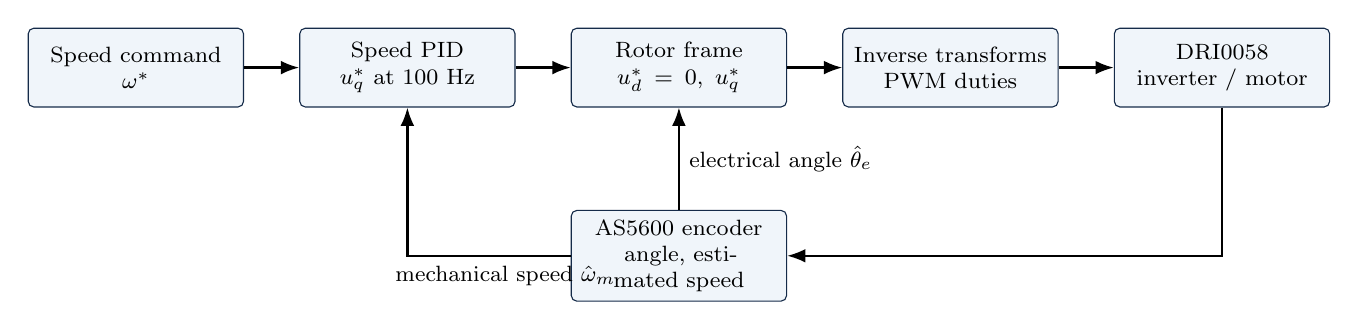
\begin{tikzpicture}[font=\footnotesize,>=Latex,node distance=7mm]
\tikzstyle{blk}=[draw=navy,fill=lightblue,rounded corners=2pt,minimum height=10mm,align=center,text width=25mm]
\node[blk] (sp) {Speed command\\$\omega^*$};
\node[blk,right=of sp] (pid) {Speed PID\\$u_q^*$ at 100 Hz};
\node[blk,right=of pid] (foc) {Rotor frame\\$u_d^*=0,\ u_q^*$};
\node[blk,right=of foc] (mod) {Inverse transforms\\PWM duties};
\node[blk,right=of mod] (drv) {DRI0058\\inverter / motor};
\draw[->,thick] (sp)--(pid);\draw[->,thick] (pid)--(foc);\draw[->,thick] (foc)--(mod);\draw[->,thick] (mod)--(drv);
\node[blk,below=13mm of foc] (sen) {AS5600 encoder\\angle, estimated speed};
\draw[->,thick] (drv.south) |- (sen.east);\draw[->,thick] (sen.west) -| node[pos=0.20,below]{mechanical speed $\hat\omega_m$} (pid.south);
\draw[->,thick] (sen.north) -- node[right]{electrical angle $\hat\theta_e$} (foc.south);
\end{tikzpicture}
\end{center}
\textbf{Two distinct frequencies:} PWM switching frequency $f_{\rm pwm}$ and FOC voltage-vector update frequency $f_{\rm foc}$ need not equal one another. The mechanical speed loop $f_v$ is slower. An illustrative design might use $f_{\rm pwm}=\SI{20}{kHz}$, $f_{\rm foc}=\SI{5}{kHz}$ and $f_v=\SI{100}{Hz}$, subject to measured encoder latency, CPU load, and hardware capability.

\section{Units, coordinates, and sign conventions}
The meaning of a $d$ or $q$ axis depends on definitions. One inconsistent $90^\circ$ shift is sufficient to turn commanded torque into flux or reverse the motor. In this note: mechanical positive rotation increases $\theta_m$; electrical angle $\theta_e=p\theta_m+\theta_0$ increases in the same sense; $d$ points along the permanent-magnet rotor flux; and $q$ is $+90^\circ$ electrically ahead of $d$. For positive $i_q$ the ideal motor produces positive electromagnetic torque. The phase sequence A-B-C and the sensor polarity must be verified on the bench.

\begin{center}
\begin{tabular}{@{}lll@{}}\toprule
Symbol & Meaning & Units\\\midrule
$p$ & number of \emph{pole pairs} & dimensionless\\
$\theta_m,\theta_e$ & mechanical and electrical rotor angles & rad\\
$\omega_m,\omega_e$ & mechanical and electrical angular velocities & rad/s\\
$\lambda_m$ & peak phase-equivalent PM flux linkage & Wb\\
$R_s,L_d,L_q$ & phase resistance, $d/q$ inductances & $\Omega$, H\\
$u_{a,b,c},i_{a,b,c}$ & phase-to-neutral voltages, phase currents & V, A\\
$u_{\alpha,\beta},u_{d,q}$ & stationary and rotating vector components & V\\
$J,B,T_L,T_e$ & inertia, viscous drag, load, electromagnetic torque & SI\\
$V_{\rm dc},d_a,d_b,d_c$ & bus voltage and PWM duty fractions & V, unitless\\\bottomrule
\end{tabular}
\end{center}
In a wye-connected motor without an accessible neutral, the \emph{controlled physical quantities} are line-to-line voltages: $u_{ab}=u_a-u_b$ and analogously. A common offset added to all three inverter terminal voltages cancels in these differences in the ideal balanced model.

\section{From three-phase variables to a rotating vector}
\subsection{Balanced sinusoidal three-phase set}
For a balanced system with no neutral current, $x_a+x_b+x_c=0$, where $x$ can represent current or the zero-sequence-free portion of voltage. A fundamental rotating field admits
\begin{equation}
\begin{bmatrix}x_a\\x_b\\x_c\end{bmatrix}
=X\begin{bmatrix}\cos\phi\\\cos(\phi-2\pi/3)\\\cos(\phi+2\pi/3)\end{bmatrix}.
\end{equation}
A single rotating two-dimensional vector is easier to control than three sinusoidal channels. Define the amplitude-invariant Clarke transform
\begin{equation}\label{eq:clarke}
\begin{bmatrix}x_\alpha\\x_\beta\end{bmatrix}
=\frac{2}{3}\begin{bmatrix}1&-\frac12&-\frac12\\0&\frac{\sqrt3}{2}&-\frac{\sqrt3}{2}\end{bmatrix}
\begin{bmatrix}x_a\\x_b\\x_c\end{bmatrix}.
\end{equation}
Then the sinusoidal set maps to $x_\alpha=X\cos\phi$, $x_\beta=X\sin\phi$. On the balanced subspace, the inverse is
\begin{equation}\label{eq:invclarke}
\begin{bmatrix}x_a\\x_b\\x_c\end{bmatrix}
=\begin{bmatrix}1&0\\-\frac12&\frac{\sqrt3}{2}\\-\frac12&-\frac{\sqrt3}{2}\end{bmatrix}
\begin{bmatrix}x_\alpha\\x_\beta\end{bmatrix}.
\end{equation}
These are \emph{amplitude invariant}, not power invariant. Therefore balanced three-phase electrical power obeys
\begin{equation}\label{eq:power}
p_e=u_ai_a+u_bi_b+u_ci_c=\frac32(u_\alpha i_\alpha+u_\beta i_\beta)=\frac32(u_di_d+u_qi_q).
\end{equation}
This factor $3/2$ propagates into the electromagnetic torque constant. A power-invariant Clarke transform uses $\sqrt{2/3}$ instead and yields different numeric component values; do not mix its equations with those in this note.

\subsection{Park transform and its inverse}
Let $c=\cos\theta_e$ and $s=\sin\theta_e$. The Park transform rotates stationary coordinates into rotor coordinates:
\begin{equation}\label{eq:park}
\begin{bmatrix}x_d\\x_q\end{bmatrix}=\underbrace{\begin{bmatrix}c&s\\-s&c\end{bmatrix}}_{R(-\theta_e)}
\begin{bmatrix}x_\alpha\\x_\beta\end{bmatrix},\qquad
\begin{bmatrix}x_\alpha\\x_\beta\end{bmatrix}=\underbrace{\begin{bmatrix}c&-s\\s&c\end{bmatrix}}_{R(+\theta_e)}
\begin{bmatrix}x_d\\x_q\end{bmatrix}.
\end{equation}
For voltage with $u_d^*=0$,
\begin{equation}\label{eq:voltagevector}
u_\alpha^*=-u_q^*\sin\theta_e,\qquad u_\beta^*=u_q^*\cos\theta_e,
\end{equation}
so the commanded stator-voltage vector lies at $\theta_e+\pi/2$. Equation \eqref{eq:voltagevector} matches the core trigonometric structure used by SimpleFOC's sinusoidal mode; library versions may distribute angle offsets and common-mode voltage differently.

\subsection{Transform invariants to test}
For any vector $\bm x$, the Park rotation preserves Euclidean norm:
\begin{equation}
x_d^2+x_q^2=x_\alpha^2+x_\beta^2,
\end{equation}
and Clarke followed by inverse Clarke reconstructs any balanced $abc$ input. Particularly useful reference cases are $\theta_e=0$, $u_d=0$, $u_q=U$ giving $(u_a,u_b,u_c)=(0,\sqrt3 U/2,-\sqrt3 U/2)$; and $\theta_e=\pi/2$ giving $(-U,U/2,U/2)$. These exact values catch most swapped-axis and sign errors.

\section{Electromechanical model derived in the rotor frame}
\subsection{Flux linkage and voltage equations}
In rotor coordinates, an ideal sinusoidal permanent-magnet synchronous machine is represented by
\begin{equation}\label{eq:flux}
\lambda_d=L_di_d+\lambda_m,\qquad \lambda_q=L_q i_q.
\end{equation}
The stator equation in stationary vector form is $\bm{u}_{\alpha\beta}=R_s\bm i_{\alpha\beta}+\dd\bm\lambda_{\alpha\beta}/\dd t$. Since $\bm\lambda_{\alpha\beta}=R(\theta_e)\bm\lambda_{dq}$, differentiate using $\dot R(\theta)=\omega_e R(\theta)\begin{psmallmatrix}0&-1\\1&0\end{psmallmatrix}$. Multiplication by $R(-\theta_e)$ gives
\begin{align}
 u_d&=R_si_d+\frac{\dd\lambda_d}{\dd t}-\omega_e\lambda_q,\\
 u_q&=R_si_q+\frac{\dd\lambda_q}{\dd t}+\omega_e\lambda_d.
\end{align}
For constant inductances and magnet flux,
\begin{align}\label{eq:dqmodel}
 u_d&=R_si_d+L_d\dot i_d-\omega_e L_qi_q,\\
 u_q&=R_si_q+L_q\dot i_q+\omega_e(L_di_d+\lambda_m).
\end{align}
The $-\omega_eL_qi_q$ and $+\omega_eL_di_d$ terms are cross-coupling; $e_q=\omega_e\lambda_m$ is the fundamental $q$-axis back-EMF. The above is a dynamical statement, not a static lookup from desired voltage to torque.

\subsection{Torque, energy conversion, and saliency}
In the amplitude-invariant convention, electrical power is $\frac32\bm u_{dq}^{\!T}\bm i_{dq}$. Isolating the speed-coupled terms from \eqref{eq:dqmodel} yields the air-gap mechanical conversion power
\begin{equation}
P_{\rm conv}=\frac32\omega_e\bigl(\lambda_di_q-\lambda_qi_d\bigr).
\end{equation}
Because $\omega_e=p\omega_m$ and $P_{\rm conv}=T_e\omega_m$,
\begin{equation}\label{eq:torque}
T_e=\frac32 p\bigl[\lambda_m i_q+(L_d-L_q)i_di_q\bigr].
\end{equation}
For a nonsalient surface-magnet rotor ($L_d\simeq L_q$), this reduces to
\begin{equation}\label{eq:Kt}
T_e=K_t i_q,\qquad K_t=\frac32 p\lambda_m.
\end{equation}
\emph{Important:} $K_t$ in \eqref{eq:Kt} is defined for this convention's \emph{peak} $q$-axis phase-current component. An RMS or line-to-line motor constant requires a conversion. For an interior PM motor, $L_d\ne L_q$ introduces reluctance torque and the optimal $i_d$ need not be zero (MTPA); that is beyond the intended hardware mode.

\subsection{Mechanical dynamics}
A useful mechanical balance is
\begin{equation}\label{eq:mech}
J\dot\omega_m=T_e-B\omega_m-T_L-T_c\operatorname{sgn}(\omega_m),\qquad \dot\theta_m=\omega_m.
\end{equation}
Here Coulomb friction $T_c$ is optional. The Phase 1 simulated plant includes inertia, linear viscous friction, and a load but \emph{not} the coupled electrical equations \eqref{eq:dqmodel}; the illustrative inertia used there is not a measurement of the FIT1035. It cannot validate a new inverter or predict actual stall current.

\section{What voltage-mode FOC does---and does not---control}
\subsection{Open-current-loop commutation with position feedback}
Sensor-based \emph{voltage mode} closes the loop around rotor \emph{position used for commutation}, while leaving both stator-current components unmeasured. The desired voltage is
\begin{equation}\label{eq:voltmode}
\bm u_{dq}^*=\begin{bmatrix}0\\u_q^*\end{bmatrix},\qquad
|u_q^*|\le U_{q,\rm lim},\qquad \bm u_{\alpha\beta}^*=R(\hat\theta_e)\bm u_{dq}^*.
\end{equation}
This is sometimes called ``torque mode: voltage'' in SimpleFOC. More precisely, $u_q$ is a signed \emph{voltage command}, not a measured current or a torque in N$\cdot$m. Actual $i_q$ and $i_d$ are whatever the motor's differential equations and load produce.

\subsection{Why $u_d=0$ does not imply $i_d=0$}
Suppose steady state ($\dot i_d=\dot i_q=0$) at nonzero electrical velocity. If $u_d=0$, the $d$-equation says
\begin{equation}\label{eq:idnotzero}
0=R_si_d-\omega_eL_qi_q\quad\Longrightarrow\quad i_d=\frac{\omega_eL_q}{R_s}i_q.
\end{equation}
Thus $i_d$ is \emph{generally nonzero} without an active $d$-axis current regulator or feedforward compensation. Equation \eqref{eq:idnotzero} is exact only for the simplified steady-state linear model, but it makes the critical point: specifying \emph{voltage} perpendicular to magnet flux is not the same as forcing \emph{current} perpendicular to magnet flux. At low $\omega_e L/R$, the difference may be modest.

\subsection{Low-speed voltage-to-current and torque approximation}
Neglect $L_d\dot i_d$, $L_q\dot i_q$ and inductive cross-coupling, with $i_d\approx0$. The $q$-equation becomes
\begin{align}\label{eq:uqiq}
u_q&\simeq R_s i_q+\omega_e\lambda_m = R_s i_q+K_e\omega_m,\quad K_e=p\lambda_m,\\
i_q&\simeq\frac{u_q-K_e\omega_m}{R_s},\qquad
T_e\simeq \frac{K_t}{R_s}(u_q-K_e\omega_m).
\end{align}
A controller with fixed $u_q$ consequently loses torque as mechanical speed and back-EMF grow. At stall, $\omega_e=0$ and $i_q\approx u_q/R_s$ after the transient: even a \emph{small} bus voltage may produce unexpectedly high copper loss if $R_s$ is small. With no current sensor, $U_{q,\rm lim}$ is not a guaranteed current limit.

\note{Do not infer a motor's electrical resistance, torque constant, or guaranteed current rating from its advertised wattage or RPM alone. The FIT1035 product data in this repository gives 12 V, 14 W, 0.8 A, and 1800 RPM, but does not establish whether the 14 W figure is mechanical output, an electrical input rating, or another catalog convention. The number $14/\omega$ is an arithmetic illustration, not a validated shaft-torque rating.}

\subsection{What changes with current-sensed FOC}
A conventional high-performance controller measures at least two phase currents and forms $i_d,i_q$ via Clarke/Park. It computes $u_d,u_q$ with two PI loops and cross-coupling compensation, and its torque command is related to measured $i_q$. This typically runs at a high rate synchronized to PWM and ADC acquisition. The DRI0058 board as specified in this project does not furnish those measurements. This note gives the equations so a reader can understand SimpleFOC's \texttt{foc\_current} mode, \emph{not} because current feedback exists in Phase 2.

\section{The inverter: voltages, modulation, and PWM}
\subsection{From an ideal space vector to real bridge terminals}
Each inverter leg is a switching half bridge. Let $d_a,d_b,d_c\in[0,1]$ be its high-side effective average duty. To first order, averaged leg-to-negative-bus voltages are $v_{a0}=\Vdc d_a$, etc. For a wye motor with floating neutral,
\begin{equation}\label{eq:terminal}
u_a=v_{a0}-v_n,\qquad v_n\approx \frac{v_{a0}+v_{b0}+v_{c0}}3.
\end{equation}
At the low-frequency fundamental, identical common-mode additions do not affect $u_{ab}$, $u_{bc}$, $u_{ca}$. This enables either sinusoidal carrier PWM (SPWM) or a space-vector-equivalent centered offset. The physical driver and wiring must implement the assumed logic polarity; active-high IN1--IN3 is documented for the DRI0058, but the pin mapping to motor phases still needs verification.

\subsection{Sinusoidal PWM with a fixed half-bus offset}
From \eqref{eq:voltagevector} and \eqref{eq:invclarke}, define zero-mean phase references $u_a^*,u_b^*,u_c^*$. The simplest three duties are
\begin{equation}\label{eq:spwm}
d_a=\frac12+\frac{u_a^*}{\Vdc},\quad
d_b=\frac12+\frac{u_b^*}{\Vdc},\quad
d_c=\frac12+\frac{u_c^*}{\Vdc}.
\end{equation}
For an arbitrary electrical angle, each of the three phase references may reach $\pm|u_q|$. To keep all duties in $[0,1]$ without clipping, one needs
\begin{equation}\label{eq:spwmlim}
\sqrt{u_d^2+u_q^2}\le\frac{\Vdc}{2},\qquad (\mathrm{linear\ SPWM}).
\end{equation}
Equation \eqref{eq:spwm} must use \emph{the bus voltage at the driver}, not the MCU supply voltage. If power supply droop is unmeasured, use a conservative calibrated bus assumption and tighter modulation bounds. Do not ``fix'' an infeasible vector by clipping each duty independently: independent clipping distorts the intended phase angles and produces torque ripple.

\subsection{Centered space-vector PWM by common-mode injection}
An elegant SVPWM construction starts from the same zero-mean phase references and adds a common-mode voltage
\begin{equation}\label{eq:svmoffset}
u_0=-\frac{\max(u_a^*,u_b^*,u_c^*)+\min(u_a^*,u_b^*,u_c^*)}{2},\qquad
d_j=\frac12+\frac{u_j^*+u_0}{\Vdc}.
\end{equation}
This centers the extrema symmetrically around $1/2$ and is equivalent to continuous, symmetric, space-vector modulation in its linear region. The duty span is
\begin{equation}
\max_j d_j-\min_j d_j=\frac{\max_j u_j^*-\min_j u_j^*}{\Vdc}.
\end{equation}
For a rotating vector of magnitude $U$, the worst-case instantaneous phase-reference span is $\sqrt3 U$. The exact linear region is therefore
\begin{equation}\label{eq:svmlim}
U=\sqrt{u_d^2+u_q^2}\le\frac{\Vdc}{\sqrt3}\approx0.577\Vdc,\qquad (\mathrm{linear\ SVPWM}).
\end{equation}
SVPWM provides $2/\sqrt3\simeq1.155$ times the linear fundamental phase amplitude of SPWM---about $15.5\%$ improvement. Both methods are modulation schemes for the \emph{same} requested fundamental voltage vector, not different FOC algorithms.

\subsection{Derivation in a 60-degree sector}
For completeness, represent the desired stationary vector over one PWM period $T_s$ by its two adjacent nonzero switching vectors $\bm V_k$ and $\bm V_{k+1}$, each of magnitude $2\Vdc/3$. If $\phi\in[0,\pi/3]$ is the angle into the sector, volt-second balance gives
\begin{equation}
\bm u^* T_s=\bm V_k T_1+\bm V_{k+1}T_2+\bm0 T_0,
\qquad T_0=T_s-T_1-T_2.
\end{equation}
Taking components along the sector axes yields
\begin{equation}\label{eq:svtimes}
\frac{T_1}{T_s}=\sqrt3\frac{U}{\Vdc}\sin\left(\frac\pi3-\phi\right),\quad
\frac{T_2}{T_s}=\sqrt3\frac{U}{\Vdc}\sin\phi,\quad
\frac{T_0}{T_s}=1-\frac{T_1+T_2}{T_s}.
\end{equation}
When $U\le\Vdc/\sqrt3$, all durations remain nonnegative for any sector. A symmetric sequence divides zero-vector time between ends of the cycle. The direct min/max construction in \eqref{eq:svmoffset} avoids a sector table yet yields the corresponding averaged duties in linear operation. It is particularly convenient for a three-input PWM driver.

\subsection{Saturation and limiting strategy}
Given $\bm u_{dq}^*$, first bound its \emph{vector norm}: $\bm u_{dq}\leftarrow\bm u_{dq}^*\min(1,U_{\rm max}/\|\bm u_{dq}^*\|)$. Then transform and add the offset. This preserves requested spatial direction. For voltage-mode $u_d=0$, a symmetric clamp $u_q\in[-U_{q,\rm lim},U_{q,\rm lim}]$ is sufficient if $U_{q,\rm lim}$ respects the relevant linear modulation bound. Allow margin for dead-time effects, transistor drops, uncertainty in $V_{dc}$, and PWM minimum pulse restrictions. Compare \emph{commanded} voltage against \emph{realizable} voltage for speed-loop anti-windup.

\subsection{Duty zero is not the same as a safe motor-off state}
Three duties at $50\%$ correspond to zero \emph{averaged line-to-line voltage} but actively switch the bridge; zero average voltage is \emph{not} zero conduction loss, zero circulating current, or open circuit. Similarly, driving all duties to 0 or 1 can connect motor phases to a common rail, causing electrical braking rather than freewheeling. Stop semantics (coast, brake, hold torque, disable) must be explicit and implemented by the actual driver power stage. On the DRI0058, the EN/RESET/SLEEP and FAULT functions must be studied and tested rather than treating numerical $u_q=0$ as a safety interlock.

\section{Electrical angle, rotor sensing, and alignment}
\subsection{Mechanical versus electrical rotation}
The motor's $p$ pole pairs imply
\begin{equation}\label{eq:angle}
\theta_e=\wrap\bigl(s\,p\,\theta_{\rm sens}+\theta_0\bigr),\quad
\omega_e=s\,p\,\omega_{\rm sens},\qquad s\in\{-1,+1\}.
\end{equation}
The sign $s$ captures relative sensor and phase-sequence orientation; $\theta_0$ captures the electrical phase reference. If the sensor angle already tracks mechanical positive orientation, $s=+1$. With $p=7$, one complete mechanical revolution maps to \emph{seven} electrical cycles. This conversion must be applied \emph{before} calculating $\sin\theta_e,\cos\theta_e$.

\subsection{AS5600 and numerical resolution}
An ideal 12-bit absolute code $n\in\{0,\dots,4095\}$ maps to
\begin{equation}
\hat\theta_{\rm sens}=\frac{2\pi n}{4096},\qquad
\Delta\theta_m=\frac{2\pi}{4096}\simeq\SI{0.08789}{\degree},\quad
\Delta\theta_e=p\Delta\theta_m\simeq\SI{0.6152}{\degree}.
\end{equation}
Resolution is not the same as sensor accuracy, bandwidth, or magnetic alignment quality. AS5600 status checks, its programmable filtering, I$^2$C bus transaction time, data-ready behavior (if applicable), angle register coherence, and possible magnet mounting errors matter. Establish the \emph{actual} update rate and latency experimentally; a loop can execute at \SI{10}{kHz} while consuming much older encoder samples.

\subsection{Angle differences and velocity estimation}
If $\theta_k\in[0,2\pi)$, the naive difference $\theta_k-\theta_{k-1}$ fails near wrap. Instead define
\begin{equation}\label{eq:wrapvel}
\Delta\theta_k=\operatorname{atan2}(\sin(\theta_k-\theta_{k-1}),\cos(\theta_k-\theta_{k-1})),\quad
\hat\omega_k^{\rm raw}=\frac{\Delta\theta_k}{t_k-t_{k-1}}.
\end{equation}
This principal-value difference assumes $|\omega_m|\Delta t<\pi$, otherwise mechanical motion aliases; do not silently violate that condition. Filter the speed for the \SI{100}{Hz} outer loop using
\begin{equation}\label{eq:lpf}
\hat\omega_k=\hat\omega_{k-1}+\alpha_k\bigl(\hat\omega_k^{\rm raw}-\hat\omega_{k-1}\bigr),\qquad
\alpha_k=\frac{\Delta t_k}{\tau_f+\Delta t_k}.
\end{equation}
An exact zero-order-hold discretization of a first-order continuous low-pass is instead $\alpha_k=1-\exp(-\Delta t_k/\tau_f)$. Choose one and test the resulting phase lag. At \SI{1}{kHz}, one encoder LSB over one sample corresponds to $2\pi/(4096\cdot0.001)\simeq\SI{1.53}{rad/s}$ or \SI{14.65}{rpm}; at \SI{100}{Hz}, about \SI{1.46}{rpm}. Higher differencing rate can make \emph{unfiltered} speed noisier for a quantized encoder.

\subsection{Alignment procedure as a constrained experiment}
Without a known $\theta_0$ and sensor sign, the mathematical transform has no physical orientation. A safe, current-limited commissioning sequence is:
\begin{enumerate}
\item With inverter \emph{disabled}, verify sensor communication and magnet status while rotating the motor by hand; observe consistent angle changes and expected wraps.
\item With a mechanically unloaded, restrained test setup and a \emph{separately validated hardware supply current limit}, command a small \emph{stationary $d$-axis} stator field at chosen electrical angle $\theta_{\rm align}$. In the stationary frame, $(u_\alpha,u_\beta)=U_{\rm align}(\cos\theta_{\rm align},\sin\theta_{\rm align})$; do \emph{not} use an uncalibrated moving $q$-axis field for first alignment.
\item Allow controlled rotor settling, read stable sensor angle $\theta_{\rm sens,align}$, and derive $\theta_0=\wrap(\theta_{\rm align}-sp\theta_{\rm sens,align})$ from the chosen conventions. If phase and sensor direction are uncertain, determine $s$ with a \emph{small, slow} commanded field sweep and explicit expected motion.
\item Disable drive. Repeat with low current in both directions; check repeatability, position error, signs, and the response to slowly varying $u_q$. Store a calibration value only after validation.
\end{enumerate}
Alignment commands can exert unexpected torque. Locking the rotor at rated current is not safe by default; if the winding resistance is unknown, first estimate or measure it safely with a current-limited instrument, then pick a conservative voltage and dwell duration.

\subsection{Latency and angle prediction}
At nonzero velocity, using a delayed angle $\hat\theta_e(t-\tau)$ creates phase error $\delta\theta_e\simeq\omega_e\tau$. A simple predictor is
\begin{equation}\label{eq:lead}
\hat\theta_e(t_a)=\wrap\left(\hat\theta_e(t_s)+\hat\omega_e(t_s)(t_a-t_s)\right),
\end{equation}
where $t_s$ is the sensor sample's effective acquisition time and $t_a$ is the PWM voltage's effective application time. At $1800$ RPM and $p=7$, $\omega_e=420\pi\approx\SI{1319.5}{rad/s}$, so \SI{100}{\micro\second} of latency is $\approx\SI{7.56}{\degree}$ electrical. Prediction helps only when sample age and velocity estimate are trustworthy; cap extrapolation age and fail safely on stale feedback.

\section{Scheduling and timing on STM32F446RE}
\subsection{The required multirate architecture}
The repository's existing outer speed task runs at \SI{100}{Hz} (TIM7). At \SI{1800}{rpm}, the mechanical frequency is \SI{30}{Hz} and electrical frequency is $pf_m=7\times30=\SI{210}{Hz}$. A \SI{100}{Hz} inner update would be \emph{below the Nyquist rate of the electrical-angle cycle} and is unsuitable for smooth commutation. A candidate \SI{5}{kHz} voltage-vector update has $5000/210\approx23.8$ updates per electrical cycle and $\Delta\theta_e\approx\SI{15.1}{\degree}$ at rated speed. A \SI{10}{kHz} update yields $\approx\SI{7.56}{\degree}$ per update. These are analysis examples, \emph{not} a proof that an I$^2$C AS5600 can deliver fresh data at those rates.

\subsection{Example clock and timer math}
The existing firmware configuration reports SYSCLK $=\SI{180}{MHz}$, APB2 $=\SI{90}{MHz}$. Under the STM32 timer clock doubling rule when an APB prescaler is not 1, an APB2 advanced timer such as TIM1 has a \emph{candidate} input clock $f_{\rm tim}=\SI{180}{MHz}$. Validate this against the exact RCC and TIM clock configuration. For a center-aligned, up/down PWM timer,
\begin{equation}\label{eq:arr}
f_{\rm pwm}\simeq\frac{f_{\rm tim}}{2(\mathrm{PSC}+1)(\mathrm{ARR}+1)}.
\end{equation}
For example, $\mathrm{PSC}=0$ and $\mathrm{ARR}\approx4499$ produce about \SI{20}{kHz}. The off-by-one convention in the exact count sequence and any repetition-counter selection should be checked against RM0390 and a scope. Channel compare registers are approximately $\mathrm{CCR}_j=\operatorname{round}(d_j(\mathrm{ARR}+1))$, with explicit clipping to supported compare values. Use all three channels of \emph{one} timer, enable compare preloads, and update them atomically at an appropriate timer event to avoid a partially old duty triplet.

\subsection{Three-PWM versus six-PWM}
For the DRI0058, the MCU supplies \emph{three input PWM signals} IN1--IN3. The board handles its underlying bridge switching. MCU-generated \emph{complementary six-channel PWM and inserted dead time} are not required \emph{at the connector interface}. This does \emph{not} mean dead time is unnecessary physically: protection and shoot-through avoidance must exist inside the driver and be verified from its design/data. A different six-input MOSFET gate-driver board generally requires complementary outputs, dead-time generation, break logic, and more elaborate synchronization.

\subsection{One safe data-flow decomposition}
\begin{center}
\begin{tabularx}{\linewidth}{@{}p{24mm}p{26mm}X@{}}\toprule
Activity & Example rate & Requirements\\\midrule
I$^2$C encoder acquire & measured / feasible & Timestamp valid completed transfer; no I$^2$C in an urgent motor-timer ISR.\\
FOC duty computation & 2--10 kHz candidate & Use latest valid angle, bounded prediction, fresh or bounded-age $u_q$, finite checks; write TIM1 CCR preloads.\\
PWM carrier & 20 kHz candidate & Timer hardware switches pins; coherent, deterministic duty latch.\\
Speed PID & 100 Hz existing & Consume filtered speed; publish signed voltage command; anti-windup.\\
Telemetry / supervisor & lower-rate tasks & Report age, faults, actual rate, timing; not the primary emergency shutoff.\\\bottomrule
\end{tabularx}
\end{center}
A high-priority timer ISR may perform bounded FOC arithmetic and write preloads without touching FreeRTOS, or notify a high-priority task if measured scheduling latency permits. Critical faults should remove bridge enable through a \emph{direct} fast path, preferably hardware gating, and latch status for later task-level reporting. STM32 NVIC priorities that call FreeRTOS \texttt{FromISR} must respect \texttt{configMAX\_SYSCALL\_INTERRUPT\_PRIORITY}; an ISR above that ceiling must not call the kernel.

\section{Discrete-time voltage FOC algorithm}
\subsection{Computation at the fast update $k$}
Assume a valid timestamped encoder angle $\hat\theta_{m,k}$, angle prediction $\hat\theta_{e,k}$, an outer-loop command $u_{q,k}^*$, the measured/assumed bus voltage $V_{dc,k}$, and a known phase sequence. The control recurrence is
\begin{align}
\hat\theta_{e,k}&=\wrap(sp\hat\theta_{m,k}+\theta_0+\hat\omega_{e,k}\tau_k),\\
\tilde u_{q,k}&=\sat\bigl(u_{q,k}^*, -U_{\lim,k},U_{\lim,k}\bigr),\qquad u_{d,k}=0,\\
u_{\alpha,k}&=-\tilde u_{q,k}\sin\hat\theta_{e,k},\qquad
u_{\beta,k}=\tilde u_{q,k}\cos\hat\theta_{e,k},\\
u_{a,k}&=u_{\alpha,k},\\
u_{b,k}&=-\frac12u_{\alpha,k}+\frac{\sqrt3}{2}u_{\beta,k},\\
u_{c,k}&=-\frac12u_{\alpha,k}-\frac{\sqrt3}{2}u_{\beta,k},\\
u_{0,k}&=\begin{cases}0,&\mathrm{SPWM},\\-\frac12(\max_j u_{j,k}+\min_j u_{j,k}),&\mathrm{SVPWM},\end{cases}\\
d_{j,k}&=\frac12+\frac{u_{j,k}+u_{0,k}}{V_{dc,k}},\qquad j\in\{a,b,c\}.
\end{align}
Before application, reject non-finite inputs; ensure $V_{dc,k}>0$; check modulation feasibility and duty bounds; and convert to CCR values. Negative $u_q$ reverses the $q$-axis vector by $\pi$ automatically through its sign, so an extra angle rotation must \emph{not} also be inserted. That convention makes forward/reverse algebra symmetric.

\subsection{A reference C++20 implementation of the mathematical core}
The following host-testable code performs \emph{only} modulation math. It does not select MCU pins, power-stage enable behavior, timing, or fault mitigation; its caller performs those steps. Constants and storage require no heap.
\begin{lstlisting}[language=C++,caption={Pure modulation core: signed voltage-mode FOC}]
#include <algorithm>
#include <cmath>
#include <optional>

struct Duties { float a, b, c; };
enum class Modulation { sine_pwm, centered_svpwm };

std::optional<Duties> voltage_foc(float uq, float theta_e,
                                   float vdc, float uq_limit,
                                   Modulation mode) noexcept {
  constexpr float kPi = 3.14159265358979323846f;
  constexpr float kRoot3Over2 = 0.86602540378443865f;
  if (!std::isfinite(uq) || !std::isfinite(theta_e) ||
      !std::isfinite(vdc) || !std::isfinite(uq_limit) ||
      vdc <= 0.0f || uq_limit < 0.0f) return std::nullopt;
  const float linear_max = (mode == Modulation::sine_pwm)
                               ? 0.5f*vdc : vdc/std::sqrt(3.0f);
  const float bound = std::min(uq_limit, linear_max);
  uq = std::clamp(uq, -bound, bound);
  theta_e = std::remainder(theta_e, 2.0f*kPi);
  const float alpha = -uq*std::sin(theta_e);
  const float beta  =  uq*std::cos(theta_e);
  const float ua = alpha;
  const float ub = -0.5f*alpha + kRoot3Over2*beta;
  const float uc = -0.5f*alpha - kRoot3Over2*beta;
  const float lo = std::min({ua,ub,uc});
  const float hi = std::max({ua,ub,uc});
  const float common = (mode == Modulation::centered_svpwm)
                           ? -0.5f*(hi+lo) : 0.0f;
  auto duty = [vdc,common](float u) {
    return std::clamp(0.5f + (u+common)/vdc, 0.0f, 1.0f);
  };
  return Duties{duty(ua), duty(ub), duty(uc)};
}
\end{lstlisting}
The final \texttt{std::clamp} is a numerical last resort, \emph{not} a substitute for respecting the linear modulation range. For safety-critical firmware, the failure path should be an explicit error/status rather than allowing an absent optional to be ignored; FPU latency and library trig runtime must be benchmarked on the Cortex-M4F. In a fixed-update ISR, a bounded lookup table or CMSIS-DSP sin/cos may be appropriate if justified by measurements.

\subsection{Timer output and coherent CCR update}
At each fast FOC release, compute all three floating duties first, then their integer CCRs, then latch them through a single known timer update scheme. Writing CCR values individually with preloads enabled does not guarantee a coherent set if an update event interleaves writes; execute within a bounded pre-update window, use DMA burst where appropriate, or explicitly stage/transfer values with a documented schedule. Oscilloscope inspection must confirm update synchrony. Optional synchronization to the PWM carrier is more important than assuming a high CPU priority alone creates simultaneity.

\subsection{Fast-path pseudocode and fault state}
\begin{lstlisting}[caption={Conceptual ISR/task split; schematic only}]
// Executed after a completed sensor transfer, not in I2C blocking code:
on_encoder_complete(raw_code, captured_time) {
  if (!sensor_status_ok || stale_or_invalid(raw_code)) fast_disable();
  else publish_timestamped_angle(raw_code, captured_time);
}

// On fast periodic release (e.g., timer event):
fast_foc_update(now) {
  if (!armed || fault_latched) { disable_bridge(); return; }
  const auto sensor = read_latest_angle_snapshot();
  if (!sensor.valid || now - sensor.time > max_age) {
    latch_fault(FEEDBACK_STALE); disable_bridge(); return;
  }
  const auto uq = read_latest_outer_voltage_command();
  if (uq.stale || !finite(uq.value)) {
    latch_fault(COMMAND_INVALID); disable_bridge(); return;
  }
  const float electrical = predict_and_align(sensor, now);
  const auto duty = voltage_foc(uq.value, electrical,
                                bus_voltage, uq_limit, modulation);
  if (!duty) { latch_fault(MODULATION_ERROR); disable_bridge(); return; }
  stage_three_ccrs_atomically(*duty);
}

// At 100 Hz, in the existing FreeRTOS control task:
speed_outer_update() {
  const float measured = filtered_mechanical_speed();
  const float uq_requested = pid_in_volts(speed_setpoint - measured);
  publish_bounded_voltage_command(uq_requested);
}
\end{lstlisting}
The actual interrupt layout may differ, but \emph{bridge disable} on invalid feedback, invalid commands, and driver FAULT cannot depend on the slow supervisor successfully waking up. A fast path also needs a watchdog or hardware fault mechanism that protects against the \emph{fast update itself failing to execute}.

\section{Outer speed loop and discrete control design}
\subsection{Small-signal plant under low-speed assumptions}
Combining \eqref{eq:mech} with \eqref{eq:uqiq} for the nonsalient, quasi-static electrical approximation and $T_c=0$ yields
\begin{equation}
J\dot\omega_m+\left(B+\frac{K_tK_e}{R_s}\right)\omega_m
=\frac{K_t}{R_s}u_q-T_L.
\end{equation}
For a small-signal voltage-to-speed transfer function,
\begin{equation}\label{eq:planttf}
G_{\omega u}(s)=\frac{\omega_m(s)}{u_q(s)}
=\frac{K_t/R_s}{Js+B+K_tK_e/R_s}.
\end{equation}
This is a useful first approximation for controller design, not an identification of the FIT1035. It neglects electrical poles, speed-dependent nonlinearities, friction, saturation, sensor lag, quantization, bus ripple, and load variation. For a real motor, measure a small safe response and identify plant parameters before expecting model-derived closed-loop bandwidth predictions to hold.

\subsection{Discrete PID with filtered derivative and anti-windup}
The existing Phase 1 PID uses a parallel form with derivative on measurement. In physical voltage units,
\begin{align}
e_k&=\omega_k^*-\hat\omega_k,\\
\nu_k&=K_p e_k+I_k-K_d \hat a_k,\\
\hat a_k&=\hat a_{k-1}+\frac{T_v}{T_f+T_v}
\left(\frac{\hat\omega_k-\hat\omega_{k-1}}{T_v}-\hat a_{k-1}\right),\\
u_{q,k}&=\sat(\nu_k,-U_{q,\lim},U_{q,\lim}).
\end{align}
Conditional integration applies $I_k=I_{k-1}+K_iT_v e_k$ only if the unconstrained output is not saturated in a direction that further increases saturation; otherwise hold the integrator (and permit recovery when error reverses). With constant sample period $T_v=\SI{0.01}{s}$, the controller gains have units $K_p$ [V/(rad/s)], $K_i$ [V/rad], and $K_d$ [V s$^2$/rad] in this convention. They are \emph{not} interchangeable with the Phase 1 normalized-torque gains. Review target ranges, integrator bounds, derivative filtering, and stop/reset semantics before commissioning.

\subsection{Bandwidth hierarchy and practical tuning}
Select mechanical velocity closed-loop bandwidth well below the achievable electrical/commutation update bandwidth, sensor bandwidth, and speed estimator bandwidth. Prefer simple PI to start (set $K_d=0$), cap $u_q$, and tune under a controlled load. Raise $K_p$ until response is stable and satisfactorily damped, then gradually add $K_i$ for load rejection. Add derivative only if the speed estimate is clean and justified. Log saturation time, error, speed, velocity-estimator delay, and FAULT state. Back-calculation anti-windup can be used instead:
\begin{equation}
I_{k+1}=I_k+T_v\{K_ie_k+K_{aw}(u_{q,k}-\nu_k)\}.
\end{equation}
The output term is dimensioned in volts; $K_{aw}$ has inverse seconds. Do not integrate on a stopped or latched-fault state. Use bumpless transfer when enabling, resetting, or changing gains.

\section{Hardware interface and protection for this project}
\subsection{Board-specific reference constraints}
\begin{center}
\begin{tabularx}{\linewidth}{@{}p{30mm}p{48mm}X@{}}\toprule
Component & Published / repository information & Design consequence\\\midrule
NUCLEO-F446RE & STM32F446RET6 Cortex-M4F, 180 MHz; USART2 on PA2/PA3; TIM7 is the existing 100 Hz release & Configure three outputs of one suitable PWM timer on verified alternate-function pins; preserve console and debug routing.\\
FIT1035 & 12 V, 14 W, rated 0.8 A, rated 1800 RPM, 7 pole pairs, star wound & Electrical frequency is 210 Hz at rated speed; do not infer winding $R,L$, inertia, or stall current from ratings.\\
AS5600 & 12-bit magnetic encoder, I$^2$C, 3.3 V & Timestamp transfers, check magnet/sensor status, handle wrap and bus errors; speed estimates require filtering.\\
DRI0058 & 8--30 V motor supply; three PWM inputs; EN, RESET, SLEEP; active-low FAULT; 2.5 A/channel \emph{max published} & Power supply is independent of USB; integrate fast enable/fault handling. A per-channel maximum is not a guaranteed safe operating current for this motor.\\\bottomrule
\end{tabularx}
\end{center}
The motor manufacturer's electrical and mechanical figures should be confirmed from the current datasheet. The DRI0058's maximum PWM rate is documented as up to \SI{200}{kHz}; this does \emph{not} specify a minimum reliable pulse, recommended EMI trade-off, inverter dynamic behavior, or an appropriate application current limit. Start from the recommended operating region of the actual driver and measure switching and thermal behavior.

\subsection{STM32 configuration checklist}
\begin{enumerate}
\item Select valid alternate-function pins for \emph{one} 3-channel advanced/general-purpose timer, confirming Nucleo header routing and current board revisions. TIM1 CH1--CH3 on candidate PA8/PA9/PA10 (AF1) is a possibility to \emph{verify} with the STM32F446 pin/AF datasheet and board schematic, not a committed pin assignment.
\item Configure center-aligned PWM, compare preloads, a documented update/repetition strategy, correct signal polarities, an inactive state at startup, and an explicit bridge-enable GPIO. When the attached driver has its own internal gate logic, do \emph{not} drive it as a six-PWM interface.
\item Configure an I$^2$C controller and pins with correct voltage levels, appropriate pullups, timeouts, and recovery; do not depend on unbounded blocking HAL I$^2$C calls from the motor-timer ISR.
\item Configure a fast fault input path. An active-low driver FAULT should latch a fault and cause an immediate electrical disable. GPIO interrupt latency is not a substitute for a driver power-stage's own cycle-by-cycle protection.
\item Keep existing TIM7/FreeRTOS outer-loop timing; add a fast release source with audited NVIC priorities, CPU budget, FPU context behavior, and jitter measurements. Use DWT/timer timestamps to measure update latency rather than assuming it from priorities.
\item Verify a USB-powered Nucleo shares \emph{signal reference ground} with encoder/driver, but motor power and return-current paths do not flow through sensitive USB or prototyping signal grounds. Proper decoupling, cable lengths, wiring gauge, fusing, polarity, and thermal paths matter.
\end{enumerate}

\subsection{Current risk in voltage mode}
A driver overcurrent trip is a last-resort protection, not a programmable motor-current controller. An external current-limited supply is helpful during controlled commissioning, but dynamic transients can exceed its steady displayed reading before it reacts. Estimate conservative stall current \emph{only after} measuring $R_{LL}$ with a suitable low-resistance method; for a balanced wye motor $R_s\approx R_{LL}/2$ when measured phase-to-phase through two windings. Then the low-speed stationary relation suggests $i_q\approx u_q/R_s$ (under the dq scaling and modeling assumptions). Stalled heating is $P_{\rm Cu}=3R_s I_{\rm phase,rms}^2=(3/2)R_s I_{\rm peak}^2$ for balanced sinusoidal currents. The actual bridge switching and current waveforms may depart from that idealization.

\note{With no phase-current measurement, software \emph{cannot enforce} a dynamic current ceiling. Establish a documented hardware-limited current, temperature and duty-cycle envelope before running the motor. Do not interpret $\pm U_q$ or driver ``2.5 A maximum per channel'' as a safe continuous phase-current limit.}

\section{Startup, operation, and fault-state machine}
An implementation should distinguish at least \texttt{DISABLED}, \texttt{PRECHECK}, \texttt{ALIGN}, \texttt{READY}, \texttt{RUN}, and latched \texttt{FAULT}. Typical transitions follow:
\begin{enumerate}
\item \texttt{DISABLED} $\rightarrow$ \texttt{PRECHECK}: command PWM inactive and EN off; verify software configuration, safe supply limits, sensor status, and bridge FAULT idle state.
\item \texttt{PRECHECK} $\rightarrow$ \texttt{ALIGN}: deliberately arm a current-limited, time-limited alignment profile under operator-supervised commissioning conditions. For a previously calibrated setup, validate calibration rather than assuming it can never change.
\item \texttt{ALIGN} $\rightarrow$ \texttt{READY}: verify repeatable offset and sign; disable bridge or hold as deliberately specified, reset speed-control integrator, set command to zero.
\item \texttt{READY} $\rightarrow$ \texttt{RUN}: start fast updates first with valid feedback, then enable the driver with consistent zero/low command and ramp the speed target.
\item \texttt{RUN} $\rightarrow$ \texttt{DISABLED}/\texttt{FAULT}: rapidly remove bridge-enable for driver fault, stale encoder, numerical error, unacceptable bus conditions, overspeed, commutation deadline failures, or explicit emergency stop; telemetry follows.
\end{enumerate}
A latched fault must require deliberate, verified reset and should never automatically restart motor motion after a watchdog reset or brownout. The specified behavior of SLEEP and RESET pins must be confirmed against the driver and any power-stage requirements; reset/sleep release timing is not a generic FOC equation.

\section{Verification strategy: numerical first, physical later}
\subsection{Host-based mathematical tests}
Before any power electronics are connected, implement property-based or exhaustive-angle tests for the pure modulation function:
\begin{enumerate}
\item Check $\theta_e=0,\pi/2,\pi,3\pi/2$ and positive/negative $u_q$ against analytic phase references; verify $u_a+u_b+u_c\approx0$ before common-mode injection.
\item Sweep all $\theta_e\in[0,2\pi)$ and $u_q$ across negative/positive bounds; assert all duties finite and within $[0,1]$; check continuity near $0\leftrightarrow2\pi$ and $u_q=0$.
\item Reconstruct terminal line-to-line voltages: $\Vdc(d_a-d_b)$ must equal $u_a^*-u_b^*$ to a numerical tolerance in the linear region for both SPWM and SVPWM.
\item Assert SPWM and SVPWM produce \emph{identical line-to-line voltages} for the same realizable vector, despite different individual duties.
\item Test $u_q$ sign inversion, $p=7$ angle periodicity, sensor reversed sign, and encoder wrap; a complete mechanical revolution must contain seven complete electrical turns.
\item Inject NaN, Inf, zero/negative bus voltage, stale sensor timestamps, and out-of-range commands. Assert a fault/disable, never uninitialized CCR values.
\end{enumerate}
\subsection{Power-off and power-limited bench validation}
\begin{enumerate}
\item Without motor supply: verify console continues operating, three MCU PWM pins toggle at the expected carrier and duty, CCR updates are coherent, EN defaults off, and FAULT is read with correct polarity.
\item With motor supply off: rotate the unpowered motor manually, capture angle code, unwrap, velocity sign, and $p=7$ multiplication. Check I$^2$C timeouts and unplugged-sensor behavior.
\item Using a conservative current-limited setup: validate supply, driver sleep/reset sequence, fault reaction, and \emph{stationary} alignment only. Watch electrical/thermal behavior, not merely software assertions.
\item Spin at a very low voltage with controlled motion and compare predicted $\theta_e$ with measured encoder changes. Log one aligned electrical cycle and direction; stop if torque oscillation or uncontrolled motion occurs.
\item Only after safe commutation: enable very low speed-loop gains and small speed reference. Observe estimated speed, $u_q$, bus voltage, command saturation, and current \emph{using external instrumentation} even though firmware lacks a phase-current controller.
\item Introduce controlled fault injection: stale encoder, FAULT assertion, overdue fast update, power interruption, and reboot. Confirm actual driver-output disable at the pins with a scope. Only then expand operating conditions gradually.
\end{enumerate}
\subsection{Measurements worth archiving}
Log STM32 clock and timer configuration, oscilloscope plots for PWM frequency/duty and coherent latching, encoder transfer latency distribution, measured time-to-disable on FAULT, FOC execution jitter, and thermal/current envelope. Preserve a clear distinction between calculated nominal values, host tests, board measurements without power, and results from an energized motor. Phase 1's simulated closed-loop step response is not an inverter validation report.

\section{Reading the SimpleFOC codebase from the theory}
SimpleFOC separates mathematical commutation, motion control, sensing, and hardware abstraction. The conceptual map is:
\begin{center}
\begin{tabularx}{\linewidth}{@{}p{48mm}X@{}}\toprule
SimpleFOC surface & Role corresponding to this note\\\midrule
\shortstack[l]{\texttt{BLDCMotor::init()}\\\texttt{initFOC()}} & Driver bring-up, sensor/phase calibration, direction and electrical-zero alignment (Sections 7, 12).\\
\shortstack[l]{\texttt{BLDCMotor::}\\\texttt{loopFOC()}} & Fast path: sensor-derived electrical angle; choose voltage/current mode; compute and apply rotating-voltage components (Sections 5, 9).\\
\shortstack[l]{\texttt{BLDCMotor::}\\\texttt{setPhaseVoltage()}} & Inverse Park/Clarke and SPWM/SVPWM/trapezoid modulation, with library-specific offsets and clipping (Sections 3, 6).\\
\shortstack[l]{\texttt{BLDCMotor::}\\\texttt{move()}} & Higher-level torque, velocity, or position loop; for this project it parallels the 100 Hz speed PID (Section 10).\\
\shortstack[l]{\texttt{BLDCDriver3PWM::}\\\texttt{setPwm()}} & Translate duty/phase-voltage commands into MCU-specific PWM output calls (Section 8).\\
\texttt{Sensor}, \texttt{MagneticSensorI2C} & Read encoder; keep track of angle, velocity, sensor direction and bus timing (Section 7).\\
\shortstack[l]{\texttt{TorqueControlType::}\\\texttt{voltage}} & Directly command $u_q$; no phase-current feedback (Section 5).\\
\shortstack[l]{\texttt{TorqueControlType::}\\\texttt{foc\_current}} & Requires actual current sensors and $d/q$ current PI loops; not supported by the specified DRI0058 interface.\\\bottomrule
\end{tabularx}
\end{center}
The current library documents a three-argument voltage method\linebreak[1] \texttt{setPhaseVoltage(Uq, Ud, angle\_el)}; older versions used\linebreak[1] \texttt{setPhaseVoltage(Uq, angle\_el)}. Likewise, legacy examples sometimes normalize the angle differently or add a $90^\circ$ offset before implementing SVPWM. Those are \emph{coordinate and library-interface conventions}, not contradictions of the physical model. When reading source, trace exactly where \texttt{zero\_electric\_angle}, \texttt{sensor\_direction}, fixed $\pi/2$ shifts, and optional PWM common mode enter. Do not transplant a single source-code line without its surrounding conventions.

A compact cross-check for an independent implementation is
\begin{equation}\label{eq:fullchain}
\boxed{\quad u_{abc}^*=C^{-1}R(\hat\theta_e)\begin{bmatrix}0\\u_q^*\end{bmatrix},\qquad
\bm d=\frac12\bm 1+\frac{\bm u_{abc}^*+u_0\bm 1}{V_{dc}}\quad}
\end{equation}
with $C^{-1}$ from \eqref{eq:invclarke} and $u_0=0$ (SPWM) or from \eqref{eq:svmoffset} (SVPWM). That expression, plus alignment and power-stage details, is sufficient to write a first-principles voltage FOC modulator without depending on SimpleFOC.

\section{Common implementation failures and diagnostic signatures}
\begin{longtable}{@{}p{36mm}p{67mm}p{59mm}@{}}\toprule
Symptom & Plausible mathematical/firmware cause & Diagnostic approach\\\midrule\endhead
Motor vibrates but does not turn & Missing pole-pair multiplier; $q$ versus $d$ swapped; bad electrical offset; two phases swapped; stale angle & Manually step electrical angle at very low voltage; verify seven cycles per mechanical turn and phase mapping.\\
Motor runs backward & Wrong phase sequence or sensor direction sign & Verify positive-angle convention and change \emph{one} sign/phase mapping at a time.\\
High current at zero speed & Stall, excessive $u_q$, $R_s$ too small, PWM duty incorrectly treated as phase voltage & Disable; measure real winding resistance and current with protected instruments; reduce limits.\\
Speed ripple or audible commutation & Slow FOC update, encoder quantization, angle latency, noncoherent CCR updates & Measure angle age/jitter and phase-duty waveforms; tune predictor and timer coherence.\\
Speed PID winds up & Voltage saturation without anti-windup or incorrect normalization & Report saturated $u_q$ in volts; stop integral accumulation while pushing deeper into saturation.\\
Asymmetric direction behavior & Offset sign error, unsigned angle arithmetic, asymmetric limiter or friction & Test $+u_q$ and $-u_q$ at matched angle; assert symmetries on host.\\
Unexpected braking on stop & All legs at equal duty or hard-off interpreted incorrectly & Define bridge coast/brake state from actual driver truth table; test disabled output behavior.\\
Resets or unstable I$^2$C & Motor return-current interference, insufficient decoupling/pullups, wiring and ground layout & Scope power rails and I$^2$C with motor supply controlled; address layout, not only software retries.\\
\bottomrule
\end{longtable}

\section{Further derivations and implementation extensions}
\subsection{Electrical current-loop regulator (not present on this hardware)}
If future hardware measures phase currents, form $i_d,i_q$ with Clarke/Park and regulate
\begin{equation}
\begin{aligned}
u_d^*&=K_{pd}(i_d^*-i_d)+K_{id}\!\int(i_d^*-i_d)\dd t-\omega_eL_qi_q,\\
u_q^*&=K_{pq}(i_q^*-i_q)+K_{iq}\!\int(i_q^*-i_q)\dd t+\omega_e(L_di_d+\lambda_m).
\end{aligned}
\end{equation}
The feedforward terms cancel idealized cross-coupling and back-EMF. Current-loop bandwidth is limited by sensing/ADC acquisition, PWM delay, computation, and the $L/R$ electrical pole. With $L_d=L_q=L$, an idealized plant from decoupled voltage to current is $1/(Ls+R_s)$. A simple PI choice for desired crossover $\omega_c$ in an ideal delay-free approximation is $K_p=L\omega_c$, $K_i=R_s\omega_c$; it must be derated and validated when sensing/filtering and PWM delays are included. This extension is not voltage-only FOC.

\subsection{Torque ripple, cogging, and nonsinusoidal back-EMF}
The equations assume sinusoidal back-EMF and a balanced fundamental model. A motor marketed ``BLDC'' may have non-sinusoidal back-EMF, geometric harmonics, cogging torque, saliency, and phase asymmetry. A sine-voltage command is still possible, but torque ripple and efficiency may differ from the ideal model. No transform or PID removes physical cogging; characterize the hardware before modifying the algorithm to compensate unmeasured harmonics.

\subsection{Parameter identification and digital implementation notes}
For a wye motor, a DC phase-to-phase resistance test involves two windings in series; account for contact resistance and heating. Estimate inductance and electrical time constants with safe excitation and appropriate instrumentation. Identify $K_e$ from open-circuit back-EMF at known speed using documented RMS/peak and line/phase conventions. Identify $J,B$ using controlled coast-down or step-response tests with load accounting. On an STM32F446's single-precision FPU, keep the fast loop in \texttt{float}, explicitly finite-check all sensor/control inputs, and avoid unbounded trig/formatting/heap work in timing-critical execution. Range reduction and wrapping matter to long-run precision and to avoiding catastrophic angle discontinuities.

\section{Independent implementation acceptance criteria}
An engineer can reasonably claim a first complete \emph{voltage-mode} FOC implementation only after demonstrating: (1) a documented consistent three-phase/dq sign convention; (2) independent tested transforms and an unclipped feasible PWM modulation; (3) validated electrical-zero alignment and direction; (4) timestamped angle measurements with a bounded staleness response; (5) a fast, coherent PWM update separate from the outer loop; (6) a safe driver enable and fast fault-disabling path; (7) verified power, current and thermal limits enforced by hardware/commissioning measures appropriate to \emph{no current feedback}; and (8) recorded physical measurements under controlled test conditions. A successful firmware build, a host sinusoid plot, or the Phase 1 simulation satisfies only parts of this list.

\section{References and primary documents}
\begingroup\sloppy
\begin{enumerate}[label={[\arabic*]},leftmargin=28pt]
\item SimpleFOC, \emph{FOC Algorithm Workflow} (v2.4 documentation), \url{https://docs.simplefoc.com/foc_implementation}. Last consulted October 2026.
\item SimpleFOC, \emph{Coordinate Transformations in FOC}, \url{https://docs.simplefoc.com/foc_theory}.
\item SimpleFOC, \emph{PWM Modulation Strategies}, \url{https://docs.simplefoc.com/pwm_modulation}.
\item SimpleFOC, \emph{Torque Control Methods in FOC}, \url{https://docs.simplefoc.com/voltage_torque_control}.
\item SimpleFOC, \emph{BLDC Driver / 3PWM and 6PWM}, \url{https://docs.simplefoc.com/bldcdriver}.
\item SimpleFOC, \emph{Arduino-FOC implementation}, \url{https://github.com/simplefoc/Arduino-FOC/blob/master/src/BLDCMotor.cpp}. For an exact source audit, pin a release/commit rather than relying on the moving \texttt{master} branch.
\item STMicroelectronics, \emph{RM0390 STM32F446xx Reference Manual}, timers, RCC, NVIC and interrupts, \url{https://www.st.com/resource/en/reference_manual/dm00135183.pdf}.
\item STMicroelectronics, \emph{Motor Control Part 5: STM32 FOC Training}, \url{https://www.st.com/content/st_com/en/support/learning/stm32-moocs/Motor-Control-Part-5-STM32-Field-Oriented-motor-control-training.html}.
\item DFRobot, \emph{FIT1035 motor information}, \url{https://wiki.dfrobot.com/fit1035/}; \emph{DRI0058 SimpleFOCmini driver}, \url{https://wiki.dfrobot.com/dri0058/}.
\item Project-specific design baseline, \emph{mtrctrl Phase 2 hardware}, \url{https://github.com/jameslavrenz/mtrctrl/blob/main/docs/phase2-hardware.md}; \emph{Control design}, \url{https://github.com/jameslavrenz/mtrctrl/blob/main/docs/control-design.md}; \emph{Architecture}, \url{https://github.com/jameslavrenz/mtrctrl/blob/main/docs/architecture.md}.
\end{enumerate}
\endgroup
\vfill
\hrule\vspace{4pt}{\footnotesize\color{gray} TN-FOC-001 --- Technical theory and prospective implementation guidance; no current-sensing or real-motor safety certification is implied.}
\end{document}
